The two \acrshortpl{IDE} relevant for this thesis are Visual Studio Code (\gls{VSCode}) and \gls{Theia}.
Both are available as editors in \gls{Gitpod} as cloud based \acrshortpl{IDE}.

\subsection{Visual Studio Code}

\Gls{VSCode} is a very popular \gls{open source} \acrshort{IDE} created by Microsoft~\cite{stackoverflowStackOverflowDeveloper2019}.
A screenshot is shown in \cref{fig:vscode-ui}.
It uses web technologies like javascript, \gls{Nodejs} and \gls{Electron} to provide an advanced text editor and tools for programming on a desktop.
Originally made only for desktop, \gls{VSCode} was later adapted to also work in a browser when \gls{GitHub}\footnote{GitHub is owned by Microsoft.} launched Codespaces~\cite{svenefftingeProductRoadmapQ1}.
\Gls{VSCode} is extensible, and allows third party developers to create extensions.
These are distributed from Microsoft's extension store: Visual Studio Marketplace\footnote{Marketplace website: \href{https://marketplace.visualstudio.com/vscode}{\nolinkurl{https://marketplace.visualstudio.com/vscode}}.}.

\paragraph{Programming languages}
One common use of extensions is to support new programming languages.
The text editor in \gls{VSCode} is a generic text editor component called \textit{Monaco}~\cite{benjaminpaseroSourceCodeOrganization2020}.
This same text editor is used for all programming languages.
For the text editor to know the keywords, suggestions and other specifics of a programming language, the extension uses a standardized protocol to inform Monaco.
This protocol is called the \acrlong{LSP}, and is described in \cref{sec:lsp}.

\begin{figure}[htbp]  % order of priority: h here, t top, b bottom, p page
  \centering
  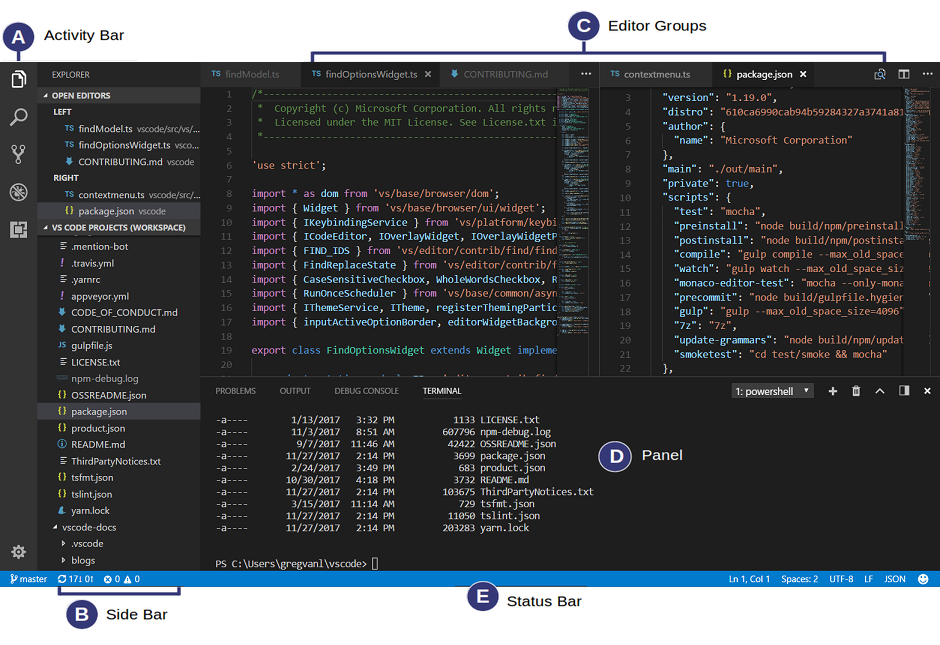
\includegraphics[width=\textwidth]{figures/pre-project/vscode-ui.png}
  \caption[VSCode User Interface]{The \gls{VSCode} user interface, annotation with the different components (A-E).}\label{fig:vscode-ui}
\end{figure}

\subsection{Theia}

Theia is based on the \gls{open source} components from \gls{VSCode}, without a proprietary component that Microsoft added for telemetry.
Theia is managed by the Eclipse Foundation, and was created to be web based from the start (before Codespaces launched, when \gls{VSCode} was desktop only).
A screenshot is shown in \cref{fig:theia-ui}.
The main uses of Theia are workspace services like \gls{Gitpod} and Eclipse Che, but it is also intended to be a ``web based version'' of the Eclipse Rich Client Platform.
This means tools can create their own distribution of Theia, where they are deeply integrated~\cite{helmingEclipseTheiaIDE2019a}.

\begin{figure}[htbp]  % order of priority: h here, t top, b bottom, p page
  \centering
  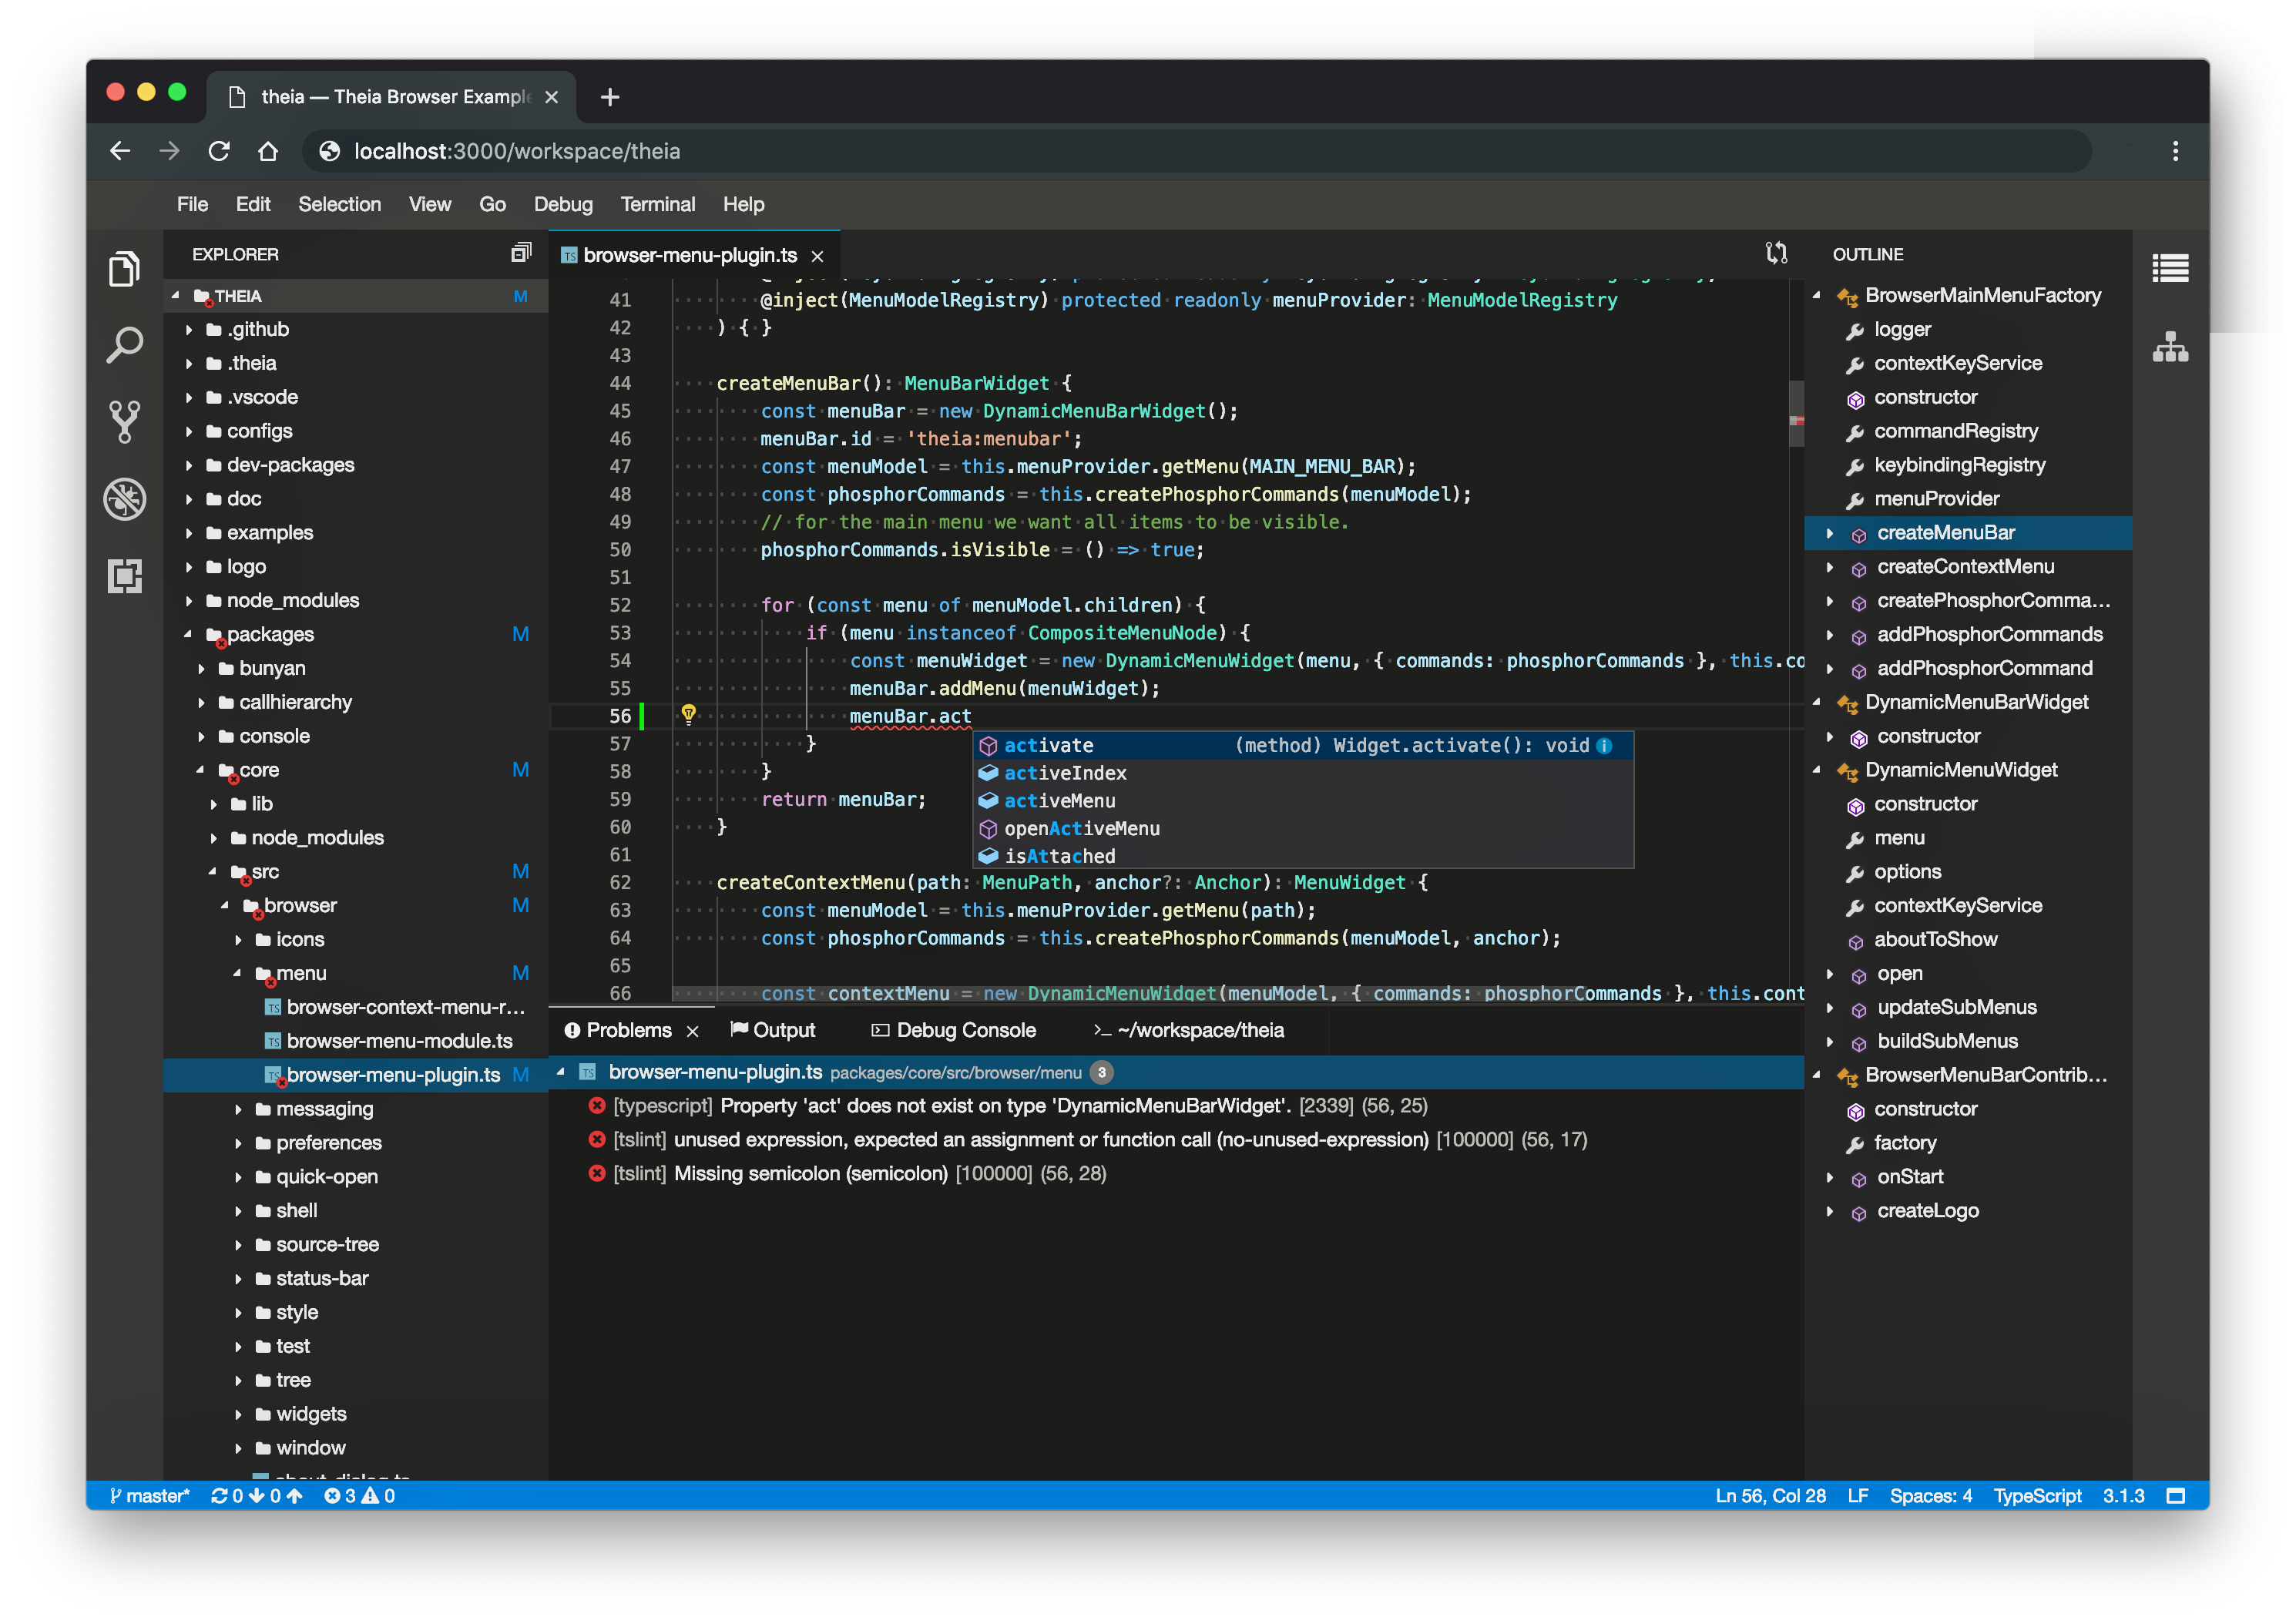
\includegraphics[width=\textwidth]{figures/pre-project/theia-screenshot.png}
  \caption[Theia User Interface]{The \gls{Theia} user interface.}\label{fig:theia-ui}
\end{figure}

\paragraph{Extensions}
Theia can load extensions using the same \acrfull{API} as \gls{VSCode}.
Theia calls these ``Theia Plugins''.
Another way to extend Theia is using ``Theia Extensions''.
These have full control over the \acrshortpl{IDE}, and can modify practically anything.
Installing a Theia Extension requires the user to perform a full compilation of \gls{Theia} itself~\cite{helmingHowAddExtensions2019}.
A Theia Plugin (or \gls{VSCode} extension) however, can be installed at runtime.
Because of licensing issues with Microsoft and the Visual Studio Marketplace, Theia Plugins are instead hosted at a independent marketplace called \textit{OpenVSX}~\cite{svenefftingeOpenVSX2020}.